\documentclass[25pt, a0paper, portrait, blockverticalspace=.5cm]{tikzposter}
\usepackage[utf8]{inputenc}
\usepackage{amssymb,amsfonts,amsmath,mathtext,mathtools}
\usepackage{xfrac}
\usepackage{enumitem}


\let\vec\oldvec
\newcommand{\vec}[1]{\boldsymbol{#1}}


\title{
	\parbox{\linewidth}{\centering
		Magneto-Optical Structure of the NICA Collider With High Critical Energy\
	}
}
\author{S.D. KOLOKOLCHIKOV\textsuperscript{1,2}, Y.V. SENICHEV\textsuperscript{1}, E.M. SYRESIN\textsuperscript{3}}
\institute{
	\textsuperscript{1} Institute for Nuclear Research of the Russian Academy of Sciences, Moscow, Russia\\
	\textsuperscript{2} Moscow Institute of Physics and Technology (MIPT), Moscow, Russia \\
	\textsuperscript{3} Joint Institute for Nuclear Researches, Dubna, Russia
}

\usetheme{Simple}
\usecolorstyle{Russia}
\colorlet{blocktitlefgcolor}{black}

\usepackage{caption}
\captionsetup{font=large}
\usepackage{multicol}
\setlength\columnsep{1.5cm}

\begin{document}

\maketitle

\begin{columns}
	\column{.5}
	\block{INTRODUCTION}{
		\par For proton option of NICA collider, it is necessary to cross the transition energy. For this reason, a magneto-optical structure with a high critical energy is considered. In this case, \\
		For NICA $\gamma_{tr} = 15$ is enough.
	}
	\column{.5}
	\block{SUPERPERIOD}{
		
		
		
		\begin{minipage}[t]{1.\linewidth}
			\begin{tikzpicture}
				\node (normal) at (0,0) {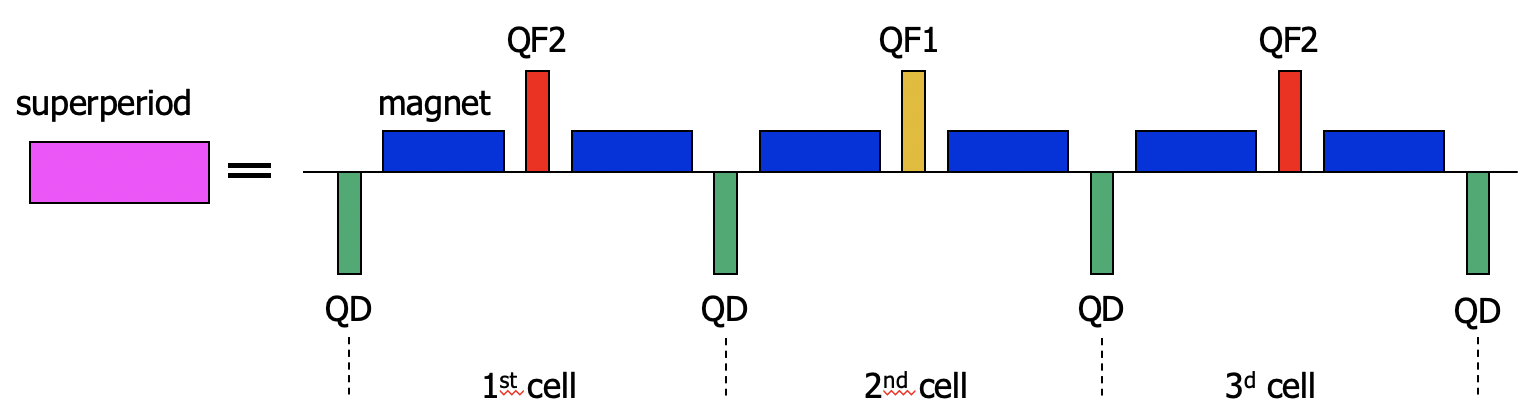
\includegraphics[width=\linewidth]{img/Superperiod}};
			\end{tikzpicture}
		\end{minipage}~~
		
		\par Expression for momentum compaction factor for a single superperiod.
		
		\par $$\alpha_{s}=\frac{1}{v_{x, \mathrm{arc}}^{2}}\left\{1+\frac{1}{4}\left(\frac{\bar{R}_{arc}}{v_{x, \text{arc}}}\right)^{4} \sum_{k=-\infty}^{\infty} \frac{g_{k}^{2}}{\left(1-k S / v_{x, \mathrm{arc}}\right)\left[1-\left(1-k S / v_{x, \mathrm{arc}}\right)^{2}\right]^{2}} \ldots\right\}$$
	}

\end{columns}

\begin{columns}
	\column{.5}
	\block{Dispersion suppression with edge cell}{
	
		\begin{minipage}{1\linewidth}
			\begin{tikzpicture}
			\node (cone) at (0,0) {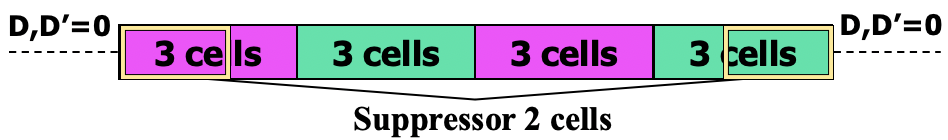
\includegraphics[width=\linewidth]{img/DS_Edge_cell}};
			\end{tikzpicture}
		\end{minipage}
		\par The dispersion suppression is carried out by using two edge FODO cells located symmetrically on both sides.\\
		
	}
	\column{.5}
	\block{2 families of quadrupoles}{
	
		\begin{minipage}{1\linewidth}
			\begin{tikzpicture}
			\node (cone) at (0,0) {\includegraphics[width=\linewidth]{img/DS_2_families}};
			\end{tikzpicture}
		\end{minipage}
		\par Dispersion Suppression by the arc, by selecting the gradients of the quadrupoles of the two families.
		
	}

\end{columns}

\begin{columns}
	\column{.5}
	\block{}{
	\begin{minipage}{1\linewidth}
			\begin{tikzpicture}
			\node (cone) at (0,0) {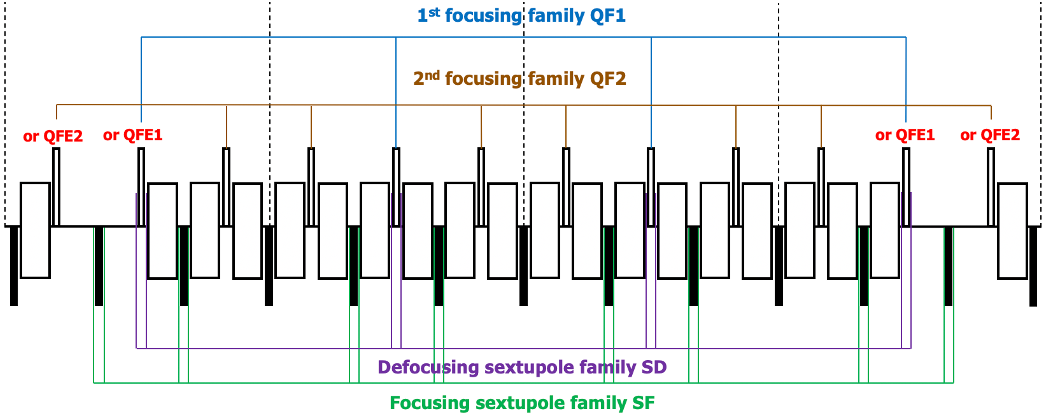
\includegraphics[width=\linewidth]{img/sextupoles_ES}};
			\end{tikzpicture}
		\end{minipage}	
	}
	\column{.5}
	\block{}{
	 
	\begin{minipage}{1\linewidth}
			\begin{tikzpicture}
			\node (cone) at (0,0) {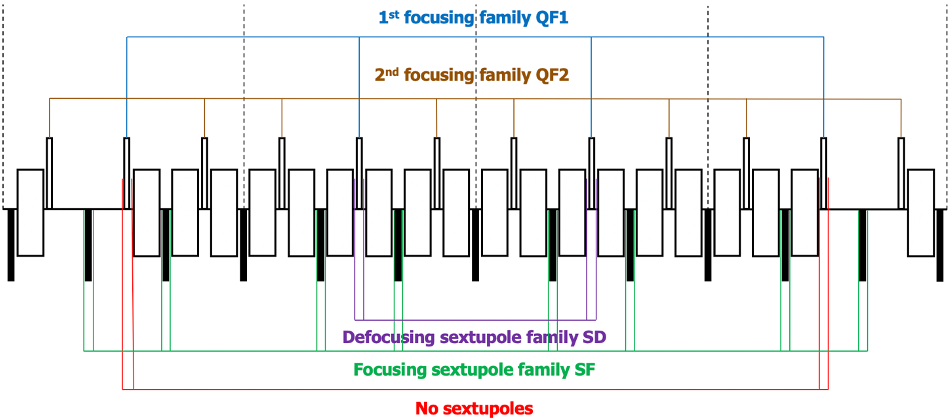
\includegraphics[width=\linewidth]{img/sextupoles_AS}};
			\end{tikzpicture}
		\end{minipage}
	}

\end{columns}

\begin{columns}
	\column{.5}
	\block{}{
	\begin{minipage}{0.5\linewidth}
			\begin{tikzpicture}
			\node (cone) at (0,0) {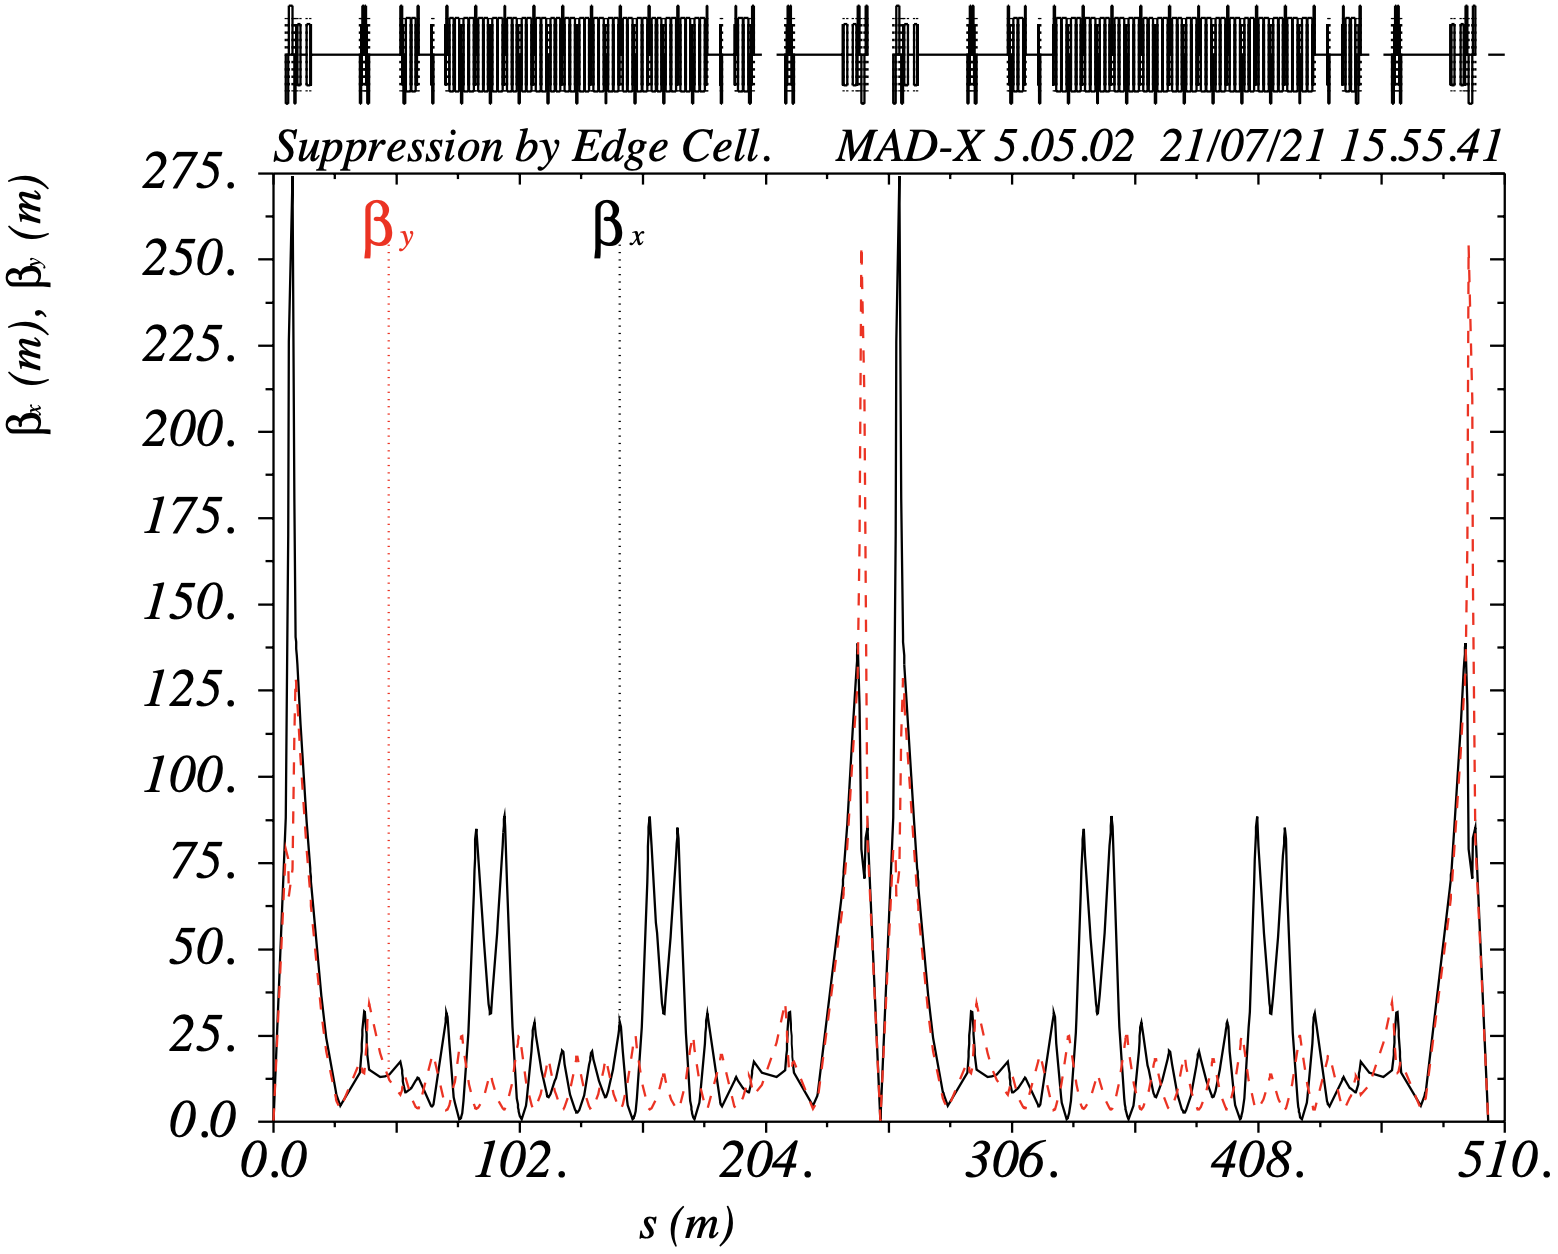
\includegraphics[width=\linewidth]{img/twiss_beta_ES}};
			\end{tikzpicture}
		\end{minipage}
		\begin{minipage}{0.5\linewidth}
			\begin{tikzpicture}
			\node (cone) at (0,0) {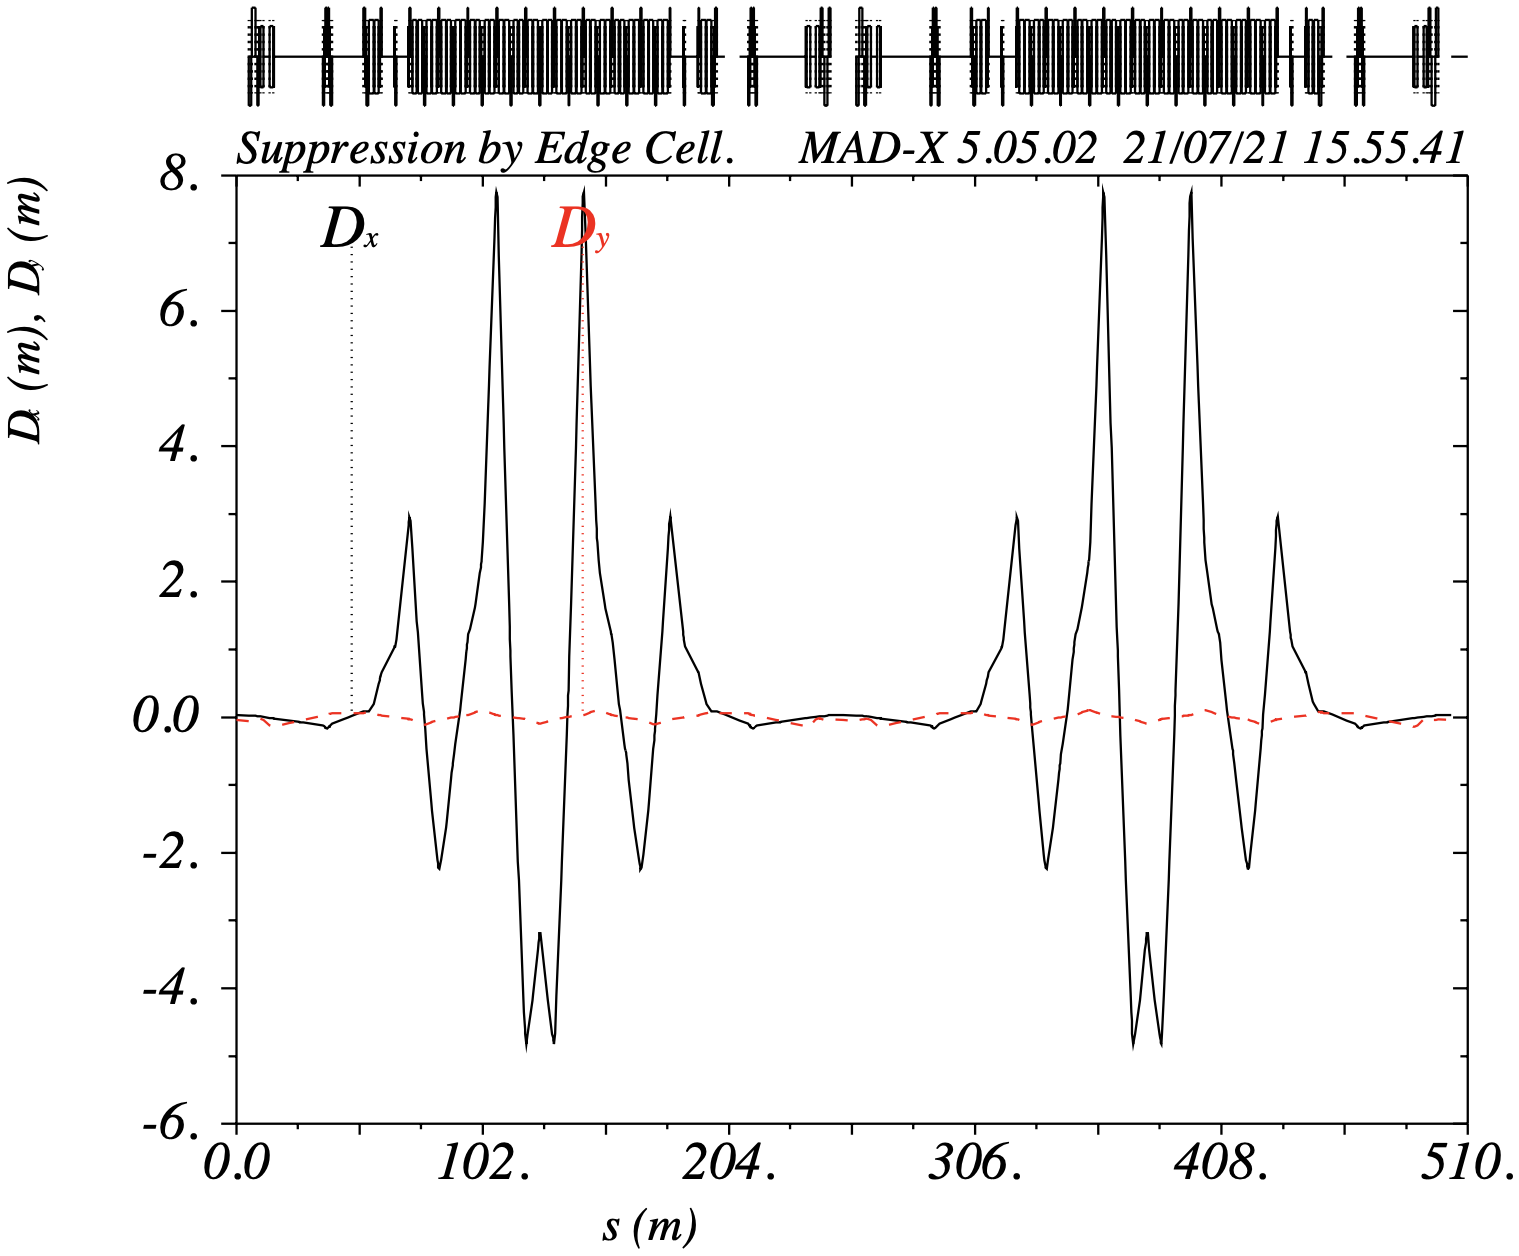
\includegraphics[width=\linewidth]{img/twiss_disp_ES}};
			\end{tikzpicture}
		\end{minipage}
		
	}
	
	\column{.5}
	\block{}{
	\begin{minipage}{0.5\linewidth}
			\begin{tikzpicture}
			\node (cone) at (0,0) {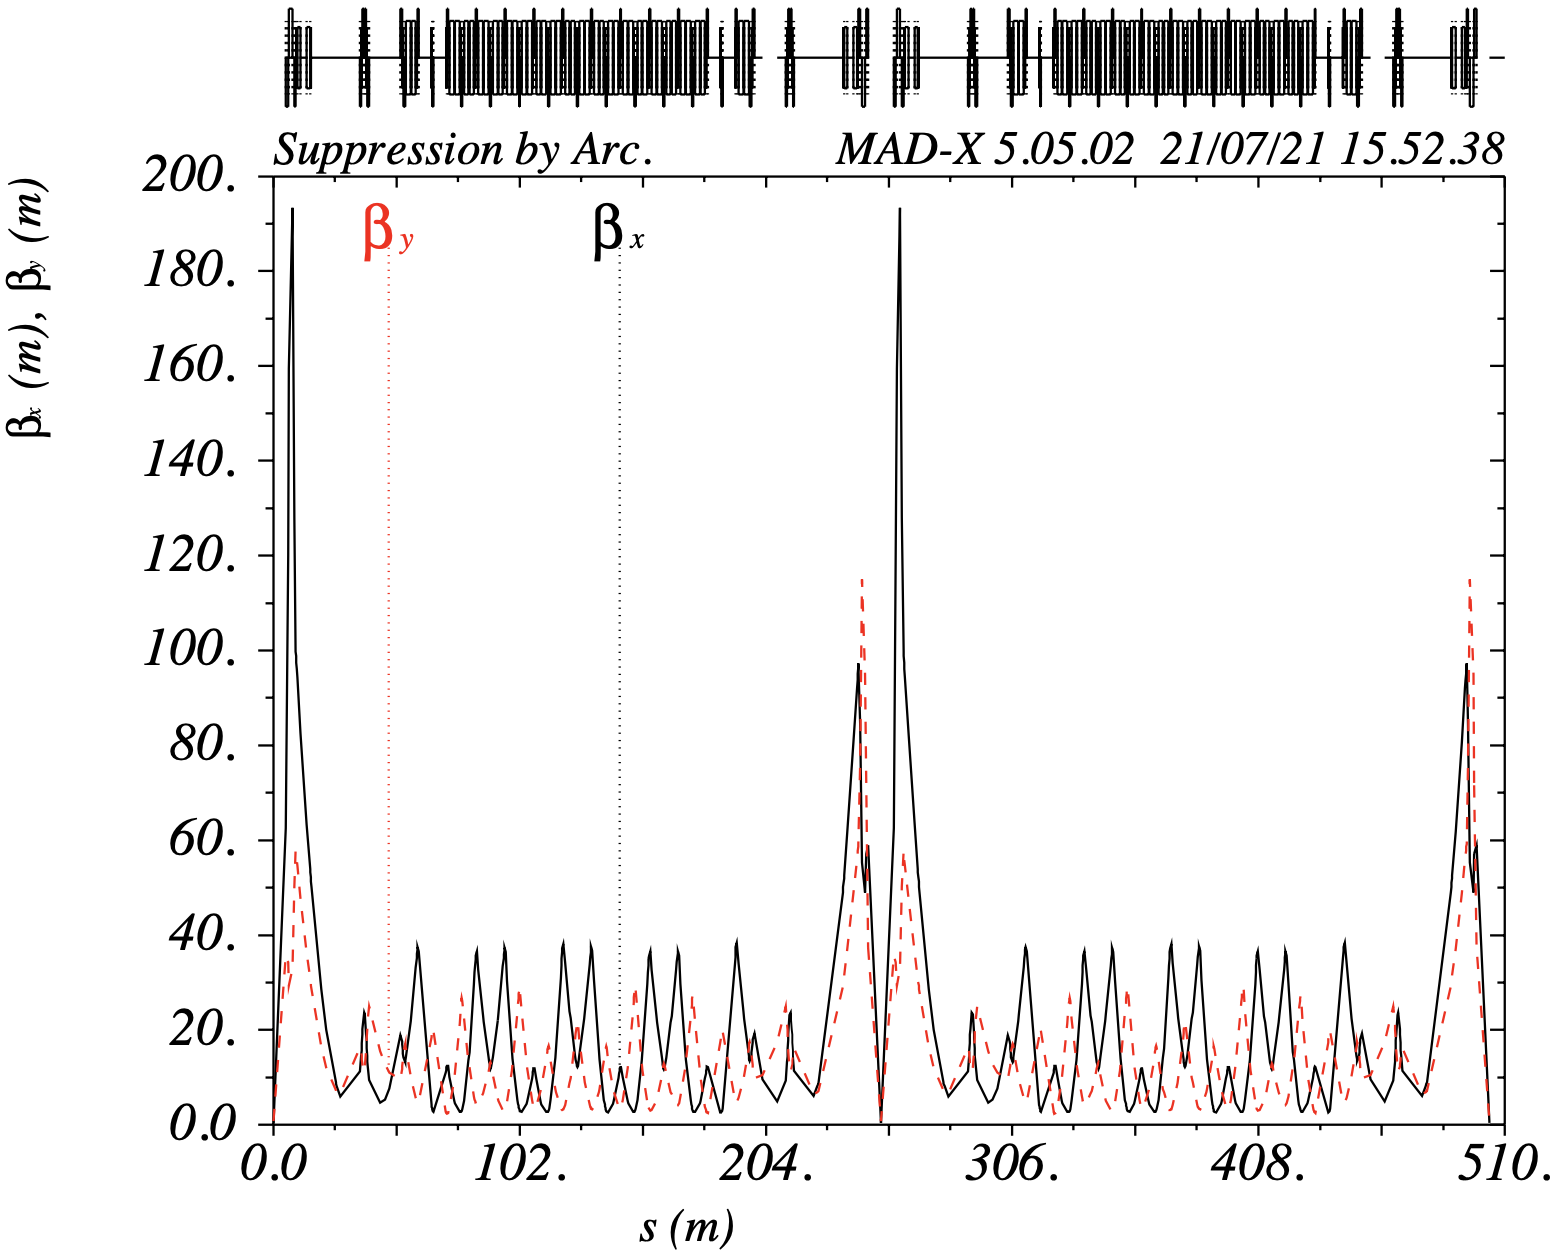
\includegraphics[width=\linewidth]{img/twiss_beta_AS}};
			\end{tikzpicture}
		\end{minipage}
		\begin{minipage}{0.5\linewidth}
			\begin{tikzpicture}
			\node (cone) at (0,0) {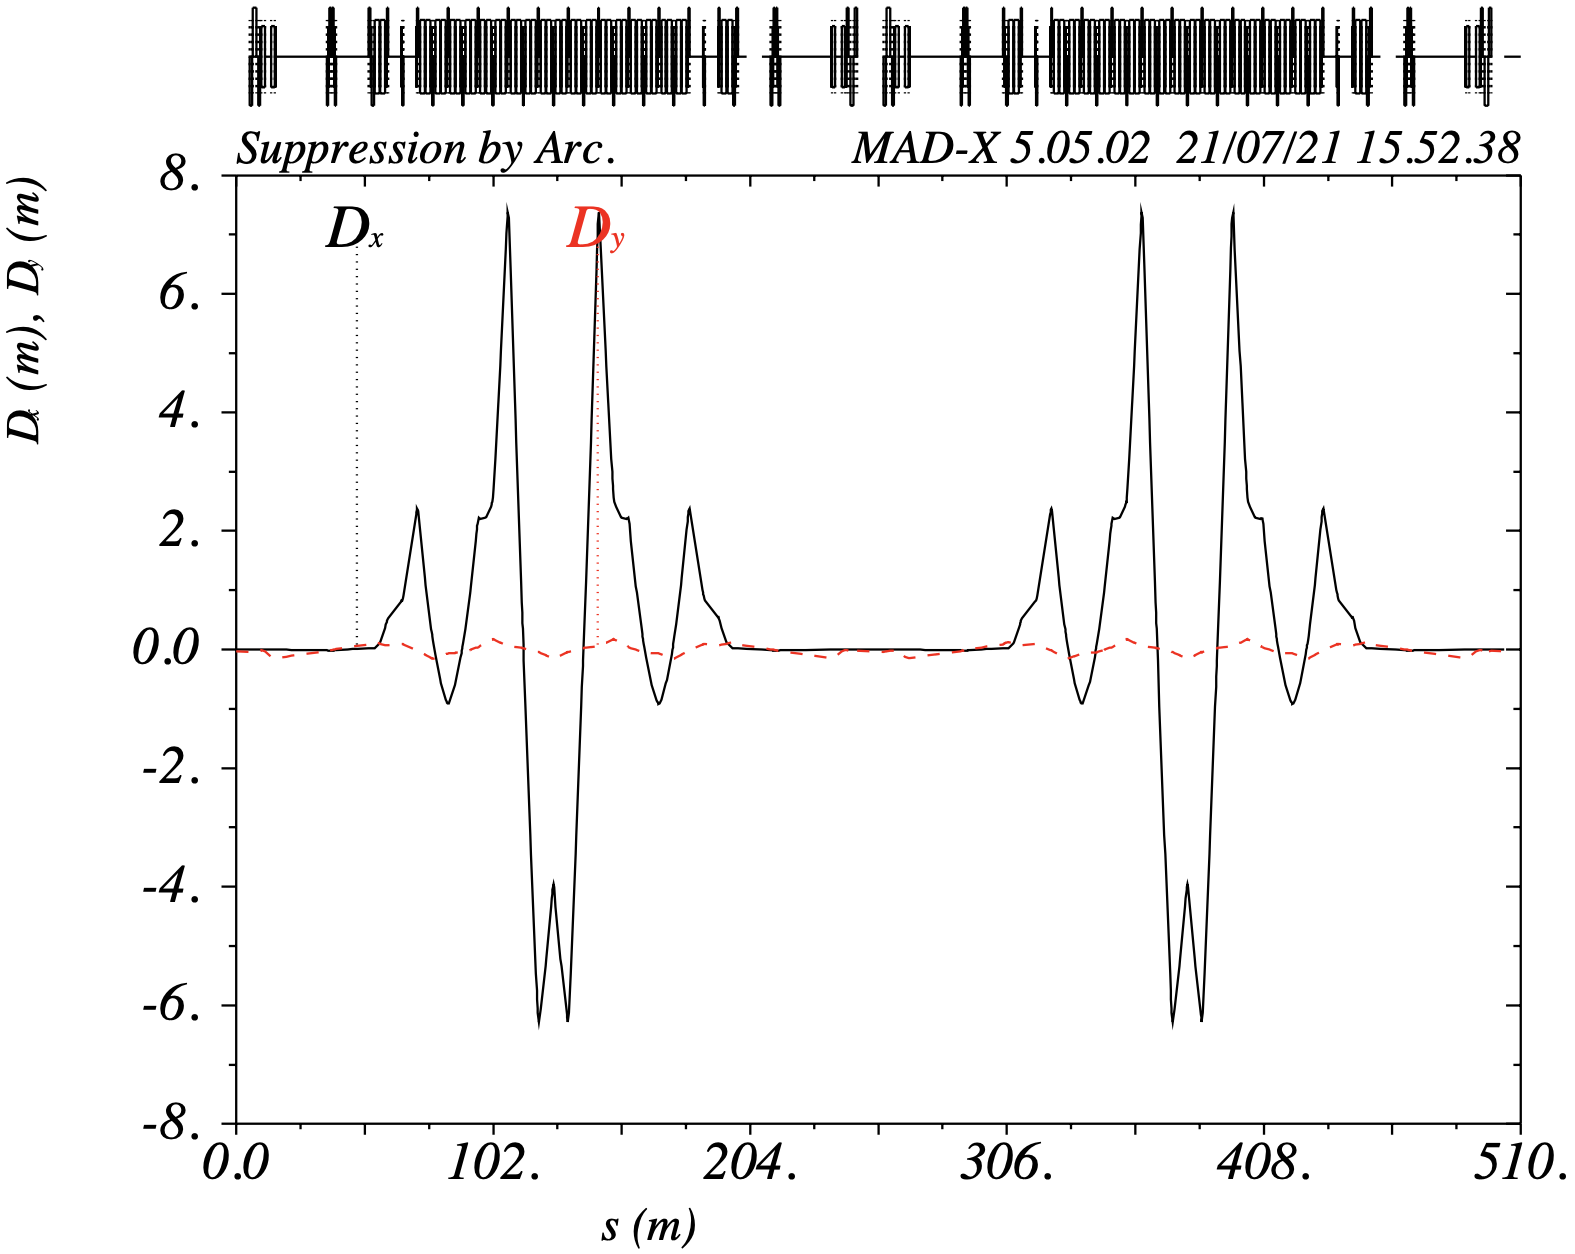
\includegraphics[width=\linewidth]{img/twiss_disp_AS}};
			\end{tikzpicture}
		\end{minipage}
		
		
	}
\end{columns}


\begin{columns}
	\column{.5}
	\block{Conclusion}{
	\par	
	}
	\column{.5}
	\block{References}{
	 
	\par 1.Yu. V. Senichev and A. N. Chechenin. Theory of “Resonant” Lattices for Synchrotrons with Negative Momentum Compaction Factor. Journal of Experimental and Theoretical Physics, 2007, Vol. 105, No. 5, pp. 988–997.
	\par 2.Yu. V. Senichev and A. N. Chechenin. Construction of “Resonant” Magneto-Optical Lattices with Controlled Momentum Compaction Factor Journal of Experimental and Theoretical Physics, 2007, Vol. 105, No. 6, pp. 1141–1156.
	}

\end{columns}

\end{document}